\subsection{Fouriertransformasjon}

Fouriertransformasjonen er en matematisk metode som brukes til å analysere 
signaler ved å dekomponere dem i deres grunnleggende frekvenskomponenter. 
Den omformer et signal fra tidsdomenet til frekvensdomenet, slik at vi kan 
identifisere hvor mye av hver frekvens som er til stede i signalet. Dette er 
nyttig for blant annet lydanalyse, filtrering og støydemping \parencite{geeksforgeeks_fourier}.

Den kontinuerlige Fouriertransformasjonen av et signal $f(t)$ er gitt ved

\begin{equation*}
    F(\omega) = \int_{-\infty}^{\infty} f(t)e^{-j\omega t}dt
\end{equation*}

hvor $F(\omega)$ representerer signalets frekvensinnhold og $\omega$ er 
vinkelfrekvensen. Den inverse transformasjonen rekonstruerer signalet tilbake til tidsdomenet:

\begin{equation*}
    f(t) = \frac{1}{2\pi} \int_{-\infty}^{\infty} F(\omega)e^{j\omega t}d\omega
\end{equation*}

Fouriertransformasjonen bryter ned signalet i en sum av sinus- og cosinusfunksjoner, 
der hver frekvens har en bestemt amplitude og fase. I vårt prosjekt brukes denne metoden 
til å analysere et lydklipp fra \textit{Seven Nation Army} av The White Stripes. 
Sangen inneholder en tydelig basslinje med frekvenser mellom omtrent 55 og 110~Hz \parencite{sevennationarmywiki}, 
noe som gjør den velegnet til å undersøke hvordan Fouriertransformasjonen kan identifisere 
dominerende frekvenser i musikk.

\subsubsection{Fourierserie}
En fourierserie brukes til å representere en periodisk funksjon som en sum av 
trigonometriske funksjoner. Dette gjør det mulig å beskrive komplekse signaler 
ved hjelp av enkle sinus- og cosinuskomponenter. For en periodisk funksjon $f(t)$ 
med periode $T$, kan funksjonen uttrykkes som en uendelig sum av eksponentielle funksjoner:

\begin{equation*}
    f(t) = \sum_{n=-\infty}^{\infty} c_n e^{j2\pi n t/T}
\end{equation*}

Koeffisientene $c_n$ angir amplituden og fasen til hver frekvenskomponent, og beregnes ved:

\begin{equation*}
    c_n = \frac{1}{T} \int_{-T/2}^{T/2} f(t)e^{-j2\pi n t/T} dt
\end{equation*}

Hver koeffisient $c_n$ viser hvor mye av frekvensen $n/T$ som er til stede i signalet. 
Når alle disse komponentene summeres, kan det opprinnelige signalet rekonstrueres nøyaktig.  

I lydanalyse betyr dette at et periodisk signal, for eksempel en tone fra \textit{Seven Nation Army}, 
kan beskrives som en kombinasjon av en grunnfrekvens og dens harmoniske overtoner. Grunnfrekvensen bestemmer tonehøyden, 
mens overtonene påvirker klangfargen og gir lyden dens karakteristiske uttrykk.


\subsubsection{Fouriertransformasjon}
Fouriertransformasjonen er en matematisk metode som brukes til å analysere 
signaler ved å dekomponere dem i deres grunnleggende frekvenskomponenter. 
Den omformer et signal fra tidsdomenet til frekvensdomenet, slik at vi kan 
identifisere hvor mye av hver frekvens som er til stede i signalet. Dette er 
nyttig for blant annet lydanalyse, filtrering og støydemping


\subsubsection{Fouriertransformasjon for vinkel­frekvens}
I mange sammenhenger uttrykkes Fouriertransformasjonen i form av \emph{vinkelfrekvens}~$\omega$ i stedet for den lineære frekvensen~$f$. Sammenhengen mellom de to er gitt ved

\begin{equation}
    \omega = 2\pi f
\end{equation}
hvor~$\omega$ måles i radianer per sekund. Ved å bruke vinkelfrekvens får man ofte enklere matematiske uttrykk, spesielt når man arbeider med eksponentialfunksjoner. Fouriertransformasjonen kan da skrives som

\begin{equation}
    F(\omega) = \int_{-\infty}^{\infty} f(t)e^{-j\omega t}\,dt
\end{equation}
og den inverse transformasjonen som

\begin{equation}
    f(t) = \frac{1}{2\pi}\int_{-\infty}^{\infty} F(\omega)e^{j\omega t}\,d\omega
\end{equation}
Denne formen brukes ofte i teoretiske analyser og i kontinuerlige modeller, mens frekvensformen~$F(f)$ oftere brukes i praktiske anvendelser, som lyd- og signalanalyse.


\subsection{Diskre Fouriertransformasjon (DFT)}
Den \emph{diskrete Fouriertransformasjonen (DFT)} brukes når signalet består av et endelig antall diskrete verdier. Dette er den formen som benyttes i digital signalbehandling, ettersom analoge signaler må samles inn som prøver (samples) for å kunne analyseres på datamaskin.

DFT-en defineres som

\begin{equation}
    X[k] = \sum_{n=0}^{N-1} x[n] e^{-j2\pi kn/N}, \quad k = 0, 1, \dots, N-1
\end{equation}
hvor~$x[n]$ er signalet i tidsdomenet og~$X[k]$ er dets representasjon i frekvensdomenet. Resultatet er periodisk med periode~$N$, og hver indeks~$k$ tilsvarer en frekvenskomponent på

\begin{equation}
    f_k = \frac{k}{N} f_s
\end{equation}
der~$f_s$ er samplingsfrekvensen. DFT gjør det mulig å analysere hvor mye energi som finnes i bestemte frekvensbånd i et digitalt signal, for eksempel hvilke frekvenser som dominerer i en musikktone.

\subsubsection{Fast Fourier Transform (FFT)}
Selv om den diskrete Fouriertransformasjonen (DFT) er konseptuelt enkel, er den beregningsmessig krevende. 
En direkte DFT-beregning krever $N^2$ multiplikasjoner, der $N$ er antall datapunkter. 
For små signaler er dette uproblematisk, men for større datamengder øker tiden raskt, og det blir upraktisk å analysere signaler i sanntid. 

Fast Fourier Transform (FFT) er en algoritme som utnytter symmetrier i DFT-formelen for å redusere antall nødvendige beregninger fra $N^2$ til $N\log_2 N$. 
Denne forbedringen gjør FFT i stand til å behandle store signaler tusenvis av ganger raskere enn en direkte DFT, uten at resultatet endres.

Anta at vi ønsker å beregne frekvensinnholdet til et signal med $N=1\,000\,000$ datapunkter.

\begin{itemize}
    \item Med DFT kreves det omtrent $N^2 = 10^{12}$ multiplikasjoner.
    \item Med FFT kreves det kun $N\log_2 N \approx 20 \times 10^6$ multiplikasjoner.
\end{itemize}

Dette betyr at FFT utfører samme analyse omtrent 50\,000 ganger raskere enn en vanlig DFT.  
Hvis en DFT-beregning tar flere minutter, vil FFT gjøre det på brøkdelen av et sekund — og det er grunnen til at 
FFT brukes i all sanntidsanalyse av lyd, kommunikasjonssignaler og bildebehandling.

\begin{figure}[H]
    \centering
    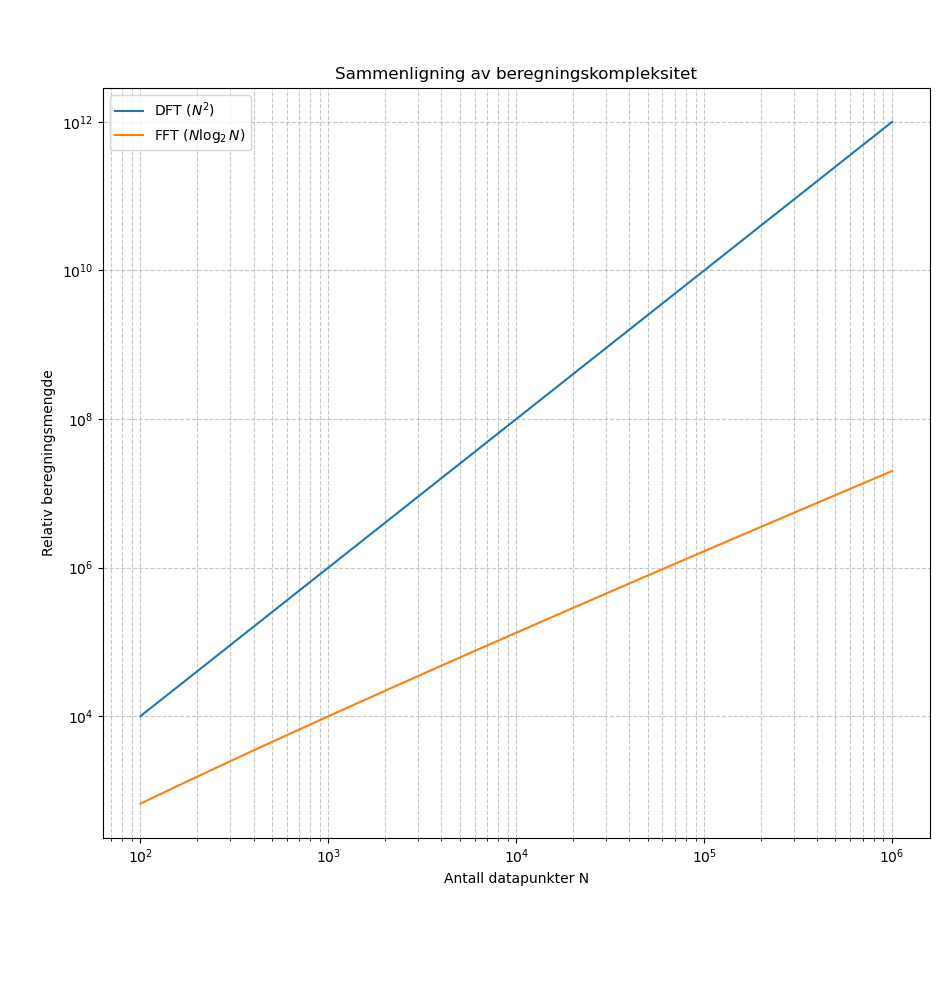
\includegraphics[width=0.85\textwidth]{figurer/fft.png}
    \caption{Beregningstid for DFT og FFT}
    \label{fig:fft_vs_dft_tidsbruk}
\end{figure}

Figuren ovenfor illustrer forskjellene i beregningstiden mellom FFT og DFT. FFT gir identisk resultat som 
DFT, men reduserer beregningstiden dramatisk. Denne effektiviteten har gjort FFT til et av de mest sentrale 
verktøyene i moderne signalbehandling.


\subsection{Short-time Fouriertransformasjon (STFT)}
\subsubsection{Kontinuerlig STFT}
Den \emph{korttids Fouriertransformasjonen} (STFT) brukes når signalets frekvensinnhold endrer seg over tid. 
I motsetning til den vanlige Fouriertransformasjonen, som viser hvilke frekvenser som finnes i hele signalet samlet, 
analyserer STFT små tidsvinduer av signalet slik at man får informasjon både om tid og frekvens samtidig \parencite{geeksforgeeks_fourier}. 

Den kontinuerlige STFT er definert som:

\begin{equation*}
    X(t,\omega) = \int_{-\infty}^{\infty} x(\tau) \, w(\tau - t) \, e^{-j\omega \tau} d\tau
\end{equation*}

hvor $x(\tau)$ er signalet og $w(\tau - t)$ er en vindusfunksjon som begrenser analysen til et kort tidsintervall. 
Valg av vindu påvirker oppløsningen: et smalt vindu gir god tidsoppløsning men dårlig frekvensoppløsning, 
mens et bredt vindu gir motsatt effekt. Dette kalles ofte et kompromiss mellom tid og frekvens \parencite{geeksforgeeks_fourier}.

I vårt prosjekt brukes STFT til å undersøke hvordan frekvensene i \textit{Seven Nation Army} varierer gjennom tid. 
Ved å beregne STFT for overlappende vinduer kan resultatet vises som et \emph{spektrogram}, 
der x-aksen viser tid, y-aksen frekvens og fargeintensiteten representerer amplituden. 
Dette gir en visuell fremstilling av hvordan ulike toner og instrumenter opptrer i sangen, 
noe som ikke er mulig å se direkte fra en vanlig Fouriertransformasjon.

\subsubsection{Diskret STFT}
Den \emph{diskrete korttids Fouriertransformasjonen} (DSTFT) brukes når signalet er digitalt representert som en rekke diskrete målepunkter. 
I praksis deles signalet inn i overlappende segmenter, og for hvert segment utføres en diskret Fouriertransformasjon (DFT eller FFT). 
Dette gir et todimensjonalt resultat som viser hvordan frekvensinnholdet endrer seg over tid.

Den diskrete STFT kan uttrykkes som

\begin{equation*}
    X(m, k) = \sum_{n=0}^{N-1} x[n + mH] \, w[n] \, e^{-j2\pi kn/N}
\end{equation*}

hvor $x[n]$ er det diskrete signalet, $w[n]$ er vindusfunksjonen, $N$ er antall punkter per vindu, og $H$ er hopplengden (antall prøver mellom hvert vindu). 
Ved å bruke en FFT-algoritme for hver vindusposisjon reduseres beregningstiden betydelig sammenlignet med direkte DFT-beregninger.

Resultatet av en diskret STFT visualiseres ofte som et \emph{spektrogram}, der man tydelig ser endringer i tonehøyde, rytme og harmonisk struktur over tid. 
I vår oppgave brukes denne metoden til å analysere lydklippet fra \textit{Seven Nation Army}, der den karakteristiske basslinjen kan observeres som tydelige 
bånd i området mellom omtrent 55 og 110~Hz. Denne fremstillingen gir et mer detaljert bilde av musikkens struktur enn den vanlige Fouriertransformasjonen.



\subsection{Sammenhengen mellom DFT, FFT og STFT}
Den diskrete Fouriertransformasjonen (DFT), Fast Fourier Transform (FFT) og Short-time Fourier Transform (STFT) er alle metoder for frekvensanalyse av signaler, 
men de brukes i forskjellige sammenhenger og har ulike egenskaper. Hovedforskjellen ligger i hvordan de behandler tidsinformasjon og beregningseffektivitet.

DFT er den grunnleggende metoden for å analysere frekvensinnholdet i et diskret signal. Den beregner frekvenskomponentene for hele signalet som en helhet, uten
tidsinformasjon. Det betyr at signalet er fast og ikke endres over tid. FFT er en effektiv algoritme for å beregne DFT raskt, noe som gjør det mulig å analysere 
store datamengder i sanntid. Dette er aktuelt fordi noen analyser krever mange transformasjoner som hadde vært vanskelig og tidkrevende med en direkte DFT-beregning.
Dette gjelder spesielt for situasjoner hvor man ikke har et komplett signal tilgjengelig på forhånd, eller når signalet endres raskt over tid. Et vanlig eksempel på 
dette er lydsignal fra seismografer som tas inn som punkter og ikke en komplett funksjon. Dette gjør at transformasjonen kun er gjennomførbar ved bruk av FFT. 
STFT, derimot, er designet for å analysere signaler som endrer seg over tid. Den deler signalet inn i små overlappende segmenter (vinduer) og utfører en DFT 
(ofte via FFT) på hvert segment. Dette gir både tids- og frekvensinformasjon, noe som er nyttig for å forstå hvordan frekvensinnholdet varierer over tid. Dette
er spesielt relevant for lydsignaler, som musikk eller tale, hvor frekvensene kan endre seg raskt.


\subsection{Alternative metoder for frekvensanalyse}
Fouriertransformasjonen og dens varianter som DFT, FFT og STFT er kraftige verktøy for frekvensanalyse, men de har også sine begrensninger, spesielt når det gjelder 
tids-frekvensoppløsning og analyse av ikke-stasjonære signaler. Derfor finnes det alternative metoder som kan være mer hensiktsmessige i visse situasjoner.
De mest kjente alternativene inkluderer Wavelet-transformasjon, Welchs metode og Wigner-Ville-distribusjon.

Wavelet-transformasjon er en metode som bruker korte bølgeformer (wavelets) for å analysere signaler på forskjellige skalaer. Dette gir bedre tids-frekvensoppløsning
sammenlignet med STFT, spesielt for signaler med raske endringer. Wavelet-transformasjon er spesielt nyttig for analyse av ikke-stasjonære signaler, som for eksempel 
biologiske signaler eller finansielle data. I motsetning til Fourier-transformasjonen, som bruker sinus- og cosinusfunksjoner, kan wavelets tilpasses for å fange opp 
både lavfrekvente og høyfrekvente komponenter mer effektivt. Dette gjør wavelet-transformasjon til et kraftig verktøy for slaglyder, korte musikalske overganger eller 
transienter. \parencite{holden_wavelets}

Welchs metode er en statistisk tilnærming for å estimere kraftspekteret til et signal. Den deler signalet inn i overlappende segmenter, beregner spekteret for hvert segment, 
og deretter gjennomsnittliggjør resultatene. Dette reduserer variansen i spekterestimatet og gir en mer pålitelig representasjon av signalets frekvensinnhold. Welchs 
metode er spesielt nyttig for støy og gir et bedre estimat av kraftspekteret enn en enkel DFT, spesielt for lange signaler med støy. Ifølge Solomon (1991), oppnås den 
reduserte variansen ved å bruke uavhengige segmenter og tilpassede vinduer (for eksempel Hann- eller Hamming-vindu), som gir en bedre estimert PSD enn et enkelt 
FFT-basert periodogram. \parencite{solomon_psd_welch_1991}

Wigner-Ville-distribusjon er en tid-frekvens representasjon som gir høy oppløsning i både tid og frekvens. Den er spesielt nyttig for analyse av signaler med
komplekse tidsvariasjoner, som for eksempel chirp-signaler eller signaler med flere frekvenskomponenter som endres over tid. Wigner-Ville-distribusjon kan imidlertid 
være utsatt for kryss-term interferens, noe som kan gjøre tolkningen av resultatene utfordrende. Ifølge McFadden (1990), gir Wigner-Ville-distribusjon en detaljert 
fremstilling av signalets energifordeling i tid-frekvens-planet, men krever nøye håndtering av krysstermene for å unngå misvisende tolkninger.
\parencite{mcfadden_intro_wigner-ville_1990}

\subsection{Vindustyper}
I både DFT- og STFT-analyse benyttes en vindusfunksjon for å begrense signalet i tid, slik at 
analysen utføres på et avgrenset segment av signalet. Valget av vindustype påvirker 
balansen mellom tids- og frekvensoppløsning, samt graden av lekkasje mellom nærliggende 
frekvenser. Denne effekten kalles \emph{spektrallekkasje} og oppstår når signalet ikke er 
nøyaktig periodisk innenfor vinduet. For å redusere lekkasje kan man benytte ulike vindustyper 
med tilpasset form og demping mot kantene.

De vanligste vindustypene er Hamming-, Hann-, Blackman- og Rectangular-vindu. 
Et rektangulært vindu gir høy frekvensoppløsning, men har samtidig sterk 
lekkasje på grunn av brå avkapping av signalet. 
Hann- og Hamming-vinduene reduserer lekkasje ved å dempe signalet gradvis mot 
kantene, men på bekostning av lavere frekvensoppløsning. 
Blackman-vinduet gir enda bedre demping av sidelobene, men sprer hovedloben mer, 
noe som reduserer presisjonen for nærliggende frekvenser. 
Valget av vindu avhenger derfor av formålet med analysen \parencite{harris_windows_1978}. 
Generelt:

\begin{itemize}
    \item Høy frekvenspresisjon: rektangulært eller Bartlett-vindu.  
    \item Lav lekkasje og jevnere spektrum: Hann-, Hamming- eller Blackman-vindu.  
\end{itemize}

I dette prosjektet benyttes et Hann-vindu, ettersom det gir en god balanse mellom tids- og 
frekvensoppløsning og reduserer spektrallekkasje tilstrekkelig for lydanalyse. 
Hann-vinduet defineres som:

\begin{equation*}
    w[n] = 0.5 \left(1 - \cos\left(\frac{2\pi n}{N-1}\right)\right), \quad 0 \leq n < N
\end{equation*}

hvor $N$ er antall prøver i vinduet.

Figur (\ref{fig:vinduer}) illustrerer forskjellen mellom noen vanlige vindustyper. 
Et godt valgt vindu sikrer at frekvensinnholdet i STFT-resultatet reflekterer de reelle 
komponentene i signalet uten unødvendige forvrengninger. \parencite{harris_windows_1978}

\begin{figure}[h]
    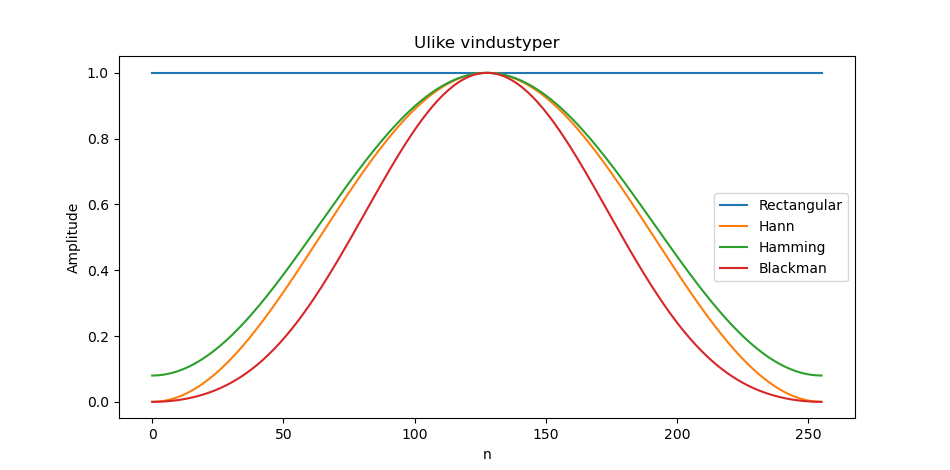
\includegraphics[width=\textwidth]{figurer/vindustyper.png}
    \label{fig:vinduer}
    \caption{Sammenligning av ulike vindustyper}
\end{figure}

Figuren ovenfor viser de vanligste vindustypene brukt ved frekvensanalyse. Den horisontale aksen ($n$) representerer antall 
prøver (tidsakse) innenfor et vindu, mens den vertikale aksen viser amplituden som signalet vektlegges med. Et rektangulært 
vindu (blå) beholder full amplitude gjennom hele vinduet, mens Hann-, Hamming- og Blackman-vinduene gradvis demper signalet 
mot kantene. Dette reduserer spektrallekkasje i Fourier-transformasjonen, men på bekostning av noe lavere frekvensoppløsning.